% Pedagogical schematic: confidence-gated, valence-asymmetric plasticity.
% Compile: pdflatex fig_plasticity.tex
\documentclass[border=8pt]{standalone}
\usepackage{amsmath,amssymb}
\usepackage{tikz}
\usetikzlibrary{arrows.meta,positioning,backgrounds,fit,calc}

\definecolor{good}{HTML}{2A7A36}
\definecolor{bad}{HTML}{B2182B}
\definecolor{ink}{HTML}{1A1A1A}
\definecolor{steel}{HTML}{1F5FA8}

% \gauge{x}{y}{frac}{color} : learning-rate bar (track + fill), width 3.4
\newcommand{\gauge}[4]{%
  \fill[black!7,rounded corners=1.6pt] (#1,#2) rectangle ++(3.4,0.32);
  \fill[#4,rounded corners=1.6pt] (#1,#2) rectangle ++({3.4*#3},0.32);
  \draw[black!22,rounded corners=1.6pt] (#1,#2) rectangle ++(3.4,0.32);}

\begin{document}
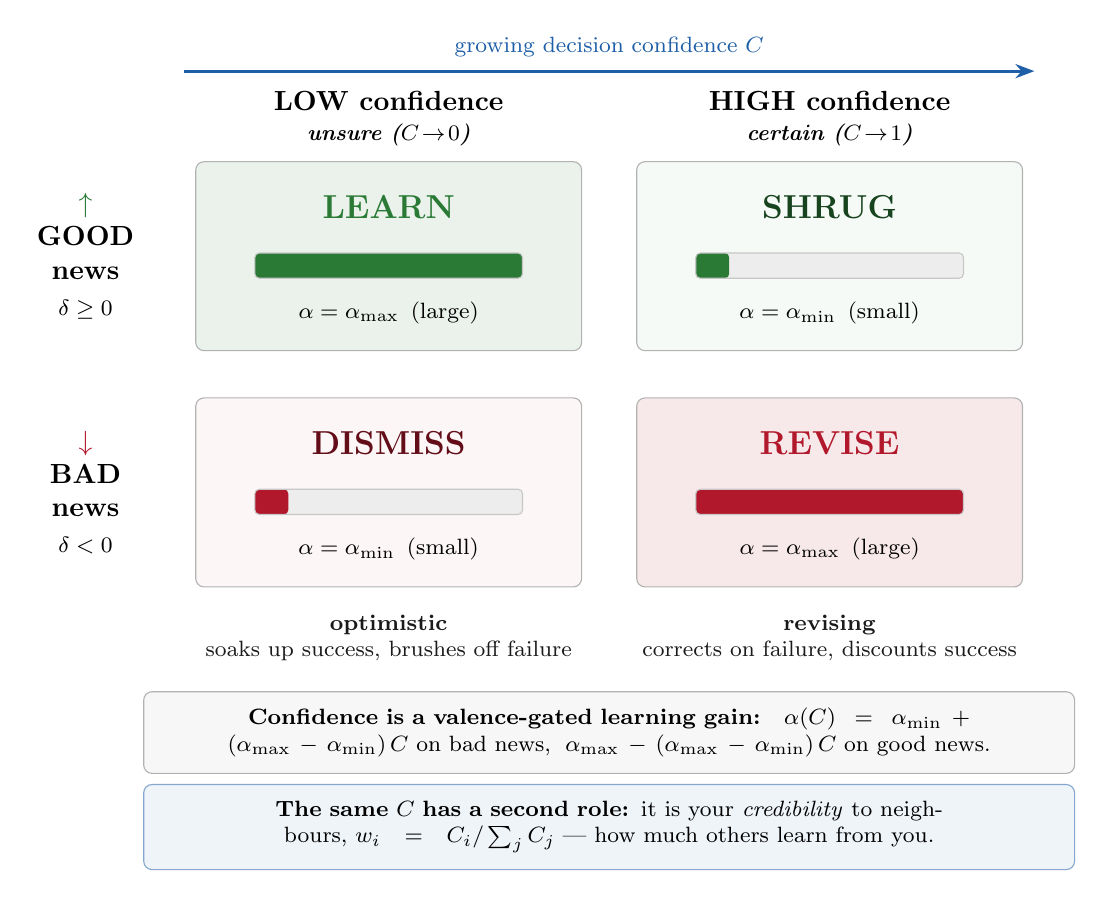
\begin{tikzpicture}[
  font=\small, >={Stealth[length=2.4mm]},
  cell/.style={rounded corners=3pt, draw=black!30, minimum width=4.9cm, minimum height=2.4cm},
  hdr/.style={font=\bfseries, align=center},
]
\def\cxL{3.1}\def\cxH{8.7}
\def\cyG{2.5}\def\cyB{-0.5}

% ===== confidence axis + column headers =====
\draw[->,line width=1pt,steel] (0.5,4.85) -- (11.3,4.85);
\node[steel,font=\footnotesize] at (5.9,5.16) {growing decision confidence $C$};
\node[hdr] at (\cxL,4.25) {LOW confidence\\[-1pt]\footnotesize\itshape unsure ($C\!\to\!0$)};
\node[hdr] at (\cxH,4.25) {HIGH confidence\\[-1pt]\footnotesize\itshape certain ($C\!\to\!1$)};

% ===== row headers =====
\node[hdr] at (-0.75,\cyG) {\textcolor{good}{$\uparrow$}\\GOOD\\news\\[1pt]\footnotesize $\delta\ge0$};
\node[hdr] at (-0.75,\cyB) {\textcolor{bad}{$\downarrow$}\\BAD\\news\\[1pt]\footnotesize $\delta<0$};

% ===== four cells =====
\node[cell,fill=good!10] (LG) at (\cxL,\cyG) {};
\node[cell,fill=good!4]  (HG) at (\cxH,\cyG) {};
\node[cell,fill=bad!4]   (LB) at (\cxL,\cyB) {};
\node[cell,fill=bad!10]  (HB) at (\cxH,\cyB) {};

% verbs + gauges + alpha
% LOW / GOOD -> big update, alpha_max
\node[font=\bfseries\large,good] at (\cxL,\cyG+0.62) {LEARN};
\gauge{\cxL-1.7}{\cyG-0.28}{1.0}{good}
\node[font=\footnotesize] at (\cxL,\cyG-0.72) {$\alpha=\alpha_{\max}$\, (large)};
% LOW / BAD -> small update, alpha_min
\node[font=\bfseries\large,bad!55!black] at (\cxL,\cyB+0.62) {DISMISS};
\gauge{\cxL-1.7}{\cyB-0.28}{0.125}{bad}
\node[font=\footnotesize] at (\cxL,\cyB-0.72) {$\alpha=\alpha_{\min}$\, (small)};
% HIGH / GOOD -> small update
\node[font=\bfseries\large,good!55!black] at (\cxH,\cyG+0.62) {SHRUG};
\gauge{\cxH-1.7}{\cyG-0.28}{0.125}{good}
\node[font=\footnotesize] at (\cxH,\cyG-0.72) {$\alpha=\alpha_{\min}$\, (small)};
% HIGH / BAD -> big update
\node[font=\bfseries\large,bad] at (\cxH,\cyB+0.62) {REVISE};
\gauge{\cxH-1.7}{\cyB-0.28}{1.0}{bad}
\node[font=\footnotesize] at (\cxH,\cyB-0.72) {$\alpha=\alpha_{\max}$\, (large)};

% ===== diagonal reading of the asymmetry =====
\node[align=center,font=\footnotesize,text=ink,text width=5cm] at (\cxL,-2.35)
  {\textbf{optimistic}\\soaks up success, brushes off failure};
\node[align=center,font=\footnotesize,text=ink,text width=5cm] at (\cxH,-2.35)
  {\textbf{revising}\\corrects on failure, discounts success};

% ===== law + social role banner =====
\node[draw=black!30,rounded corners=3pt,fill=black!3,inner sep=6pt,
      text width=11.4cm,align=center,font=\footnotesize] at (5.9,-3.55)
  {\textbf{Confidence is a valence-gated learning gain:}\quad
   $\alpha(C)=\alpha_{\min}+(\alpha_{\max}-\alpha_{\min})\,C$ on bad news,\;
   $\alpha_{\max}-(\alpha_{\max}-\alpha_{\min})\,C$ on good news.};
\node[draw=steel!55,rounded corners=3pt,fill=steel!7,inner sep=6pt,
      text width=11.4cm,align=center,font=\footnotesize] at (5.9,-4.75)
  {\textbf{The same $C$ has a second role:} it is your \emph{credibility} to
   neighbours, $w_i=C_i/\sum_j C_j$ --- how much others learn from you.};
\end{tikzpicture}
\end{document}
